% =======================================================================================================
\section{O conjunto de dados Iris}
\label{sec:dados}

\subsection{Origem e estrutura}

O conjunto Iris reúne 150 observações, 50 por espécie. Cada observação tem quatro atributos
contínuos, medidos em centímetros, e um rótulo com a espécie. A base é distribuída com a biblioteca
scikit-learn \cite{pedregosa2011} por meio da função \texttt{load\_iris}, que retorna uma matriz
$X \in \R^{150 \times 4}$ e um vetor de rótulos $y \in \{0,1,2\}^{150}$, além dos nomes das
classes. A mesma base pode ser visualizada no exemplo oficial da documentação
\cite{sklearn-iris}.

\begin{table}[htbp]
	\centering
	\caption{Estatísticas descritivas dos quatro atributos, em centímetros ($n=150$).}
	\label{tab:estatisticas}
	% gerado automaticamente por mlp_iris.py - nao editar

\begin{tabular}{lrrrrr}
\toprule
\textbf{atributo} & \textbf{média} & \textbf{desvio} & \textbf{mínimo} & \textbf{mediana} & \textbf{máximo} \\
\midrule
comp. sépala & 5{,}84 & 0{,}83 & 4{,}30 & 5{,}80 & 7{,}90 \\
larg. sépala & 3{,}06 & 0{,}44 & 2{,}00 & 3{,}00 & 4{,}40 \\
comp. pétala & 3{,}76 & 1{,}77 & 1{,}00 & 4{,}35 & 6{,}90 \\
larg. pétala & 1{,}20 & 0{,}76 & 0{,}10 & 1{,}30 & 2{,}50 \\
\bottomrule
\end{tabular}

\end{table}

\begin{table}[htbp]
	\centering
	\caption{Média $\pm$ desvio-padrão de cada atributo por espécie (cm).}
	\label{tab:estatisticas-classe}
	% gerado automaticamente por mlp_iris.py - nao editar

\begin{tabular}{lccc}
\toprule
\textbf{atributo} & \textbf{setosa} & \textbf{versicolor} & \textbf{virginica} \\
\midrule
comp. sépala & 5{,}01 $\pm$ 0{,}35 & 5{,}94 $\pm$ 0{,}52 & 6{,}59 $\pm$ 0{,}64 \\
larg. sépala & 3{,}43 $\pm$ 0{,}38 & 2{,}77 $\pm$ 0{,}31 & 2{,}97 $\pm$ 0{,}32 \\
comp. pétala & 1{,}46 $\pm$ 0{,}17 & 4{,}26 $\pm$ 0{,}47 & 5{,}55 $\pm$ 0{,}55 \\
larg. pétala & 0{,}25 $\pm$ 0{,}11 & 1{,}33 $\pm$ 0{,}20 & 2{,}03 $\pm$ 0{,}27 \\
\bottomrule
\end{tabular}

\end{table}

A \tabela{tab:estatisticas} mostra que os atributos têm escalas parecidas: o comprimento da sépala
varia de 4,3 a 7,9\,cm, enquanto a largura da pétala varia de 0,1 a 2,5\,cm. A
\tabela{tab:estatisticas-classe} revela o padrão central do problema. As dimensões da pétala
crescem de forma monótona com a espécie: a largura média da pétala é $0{,}25$\,cm na
\emph{setosa}, $1{,}33$\,cm na \emph{versicolor} e $2{,}03$\,cm na \emph{virginica}. Já a largura
da sépala \emph{não} cresce: a \emph{setosa} tem a maior média ($3{,}43$\,cm) e a
\emph{versicolor} a menor ($2{,}77$\,cm).

\subsection{Análise exploratória}

A \figura{fig:dispersao} apresenta a matriz de dispersão completa. Três aspectos merecem atenção.

\begin{figure}[ht]
	\centering
	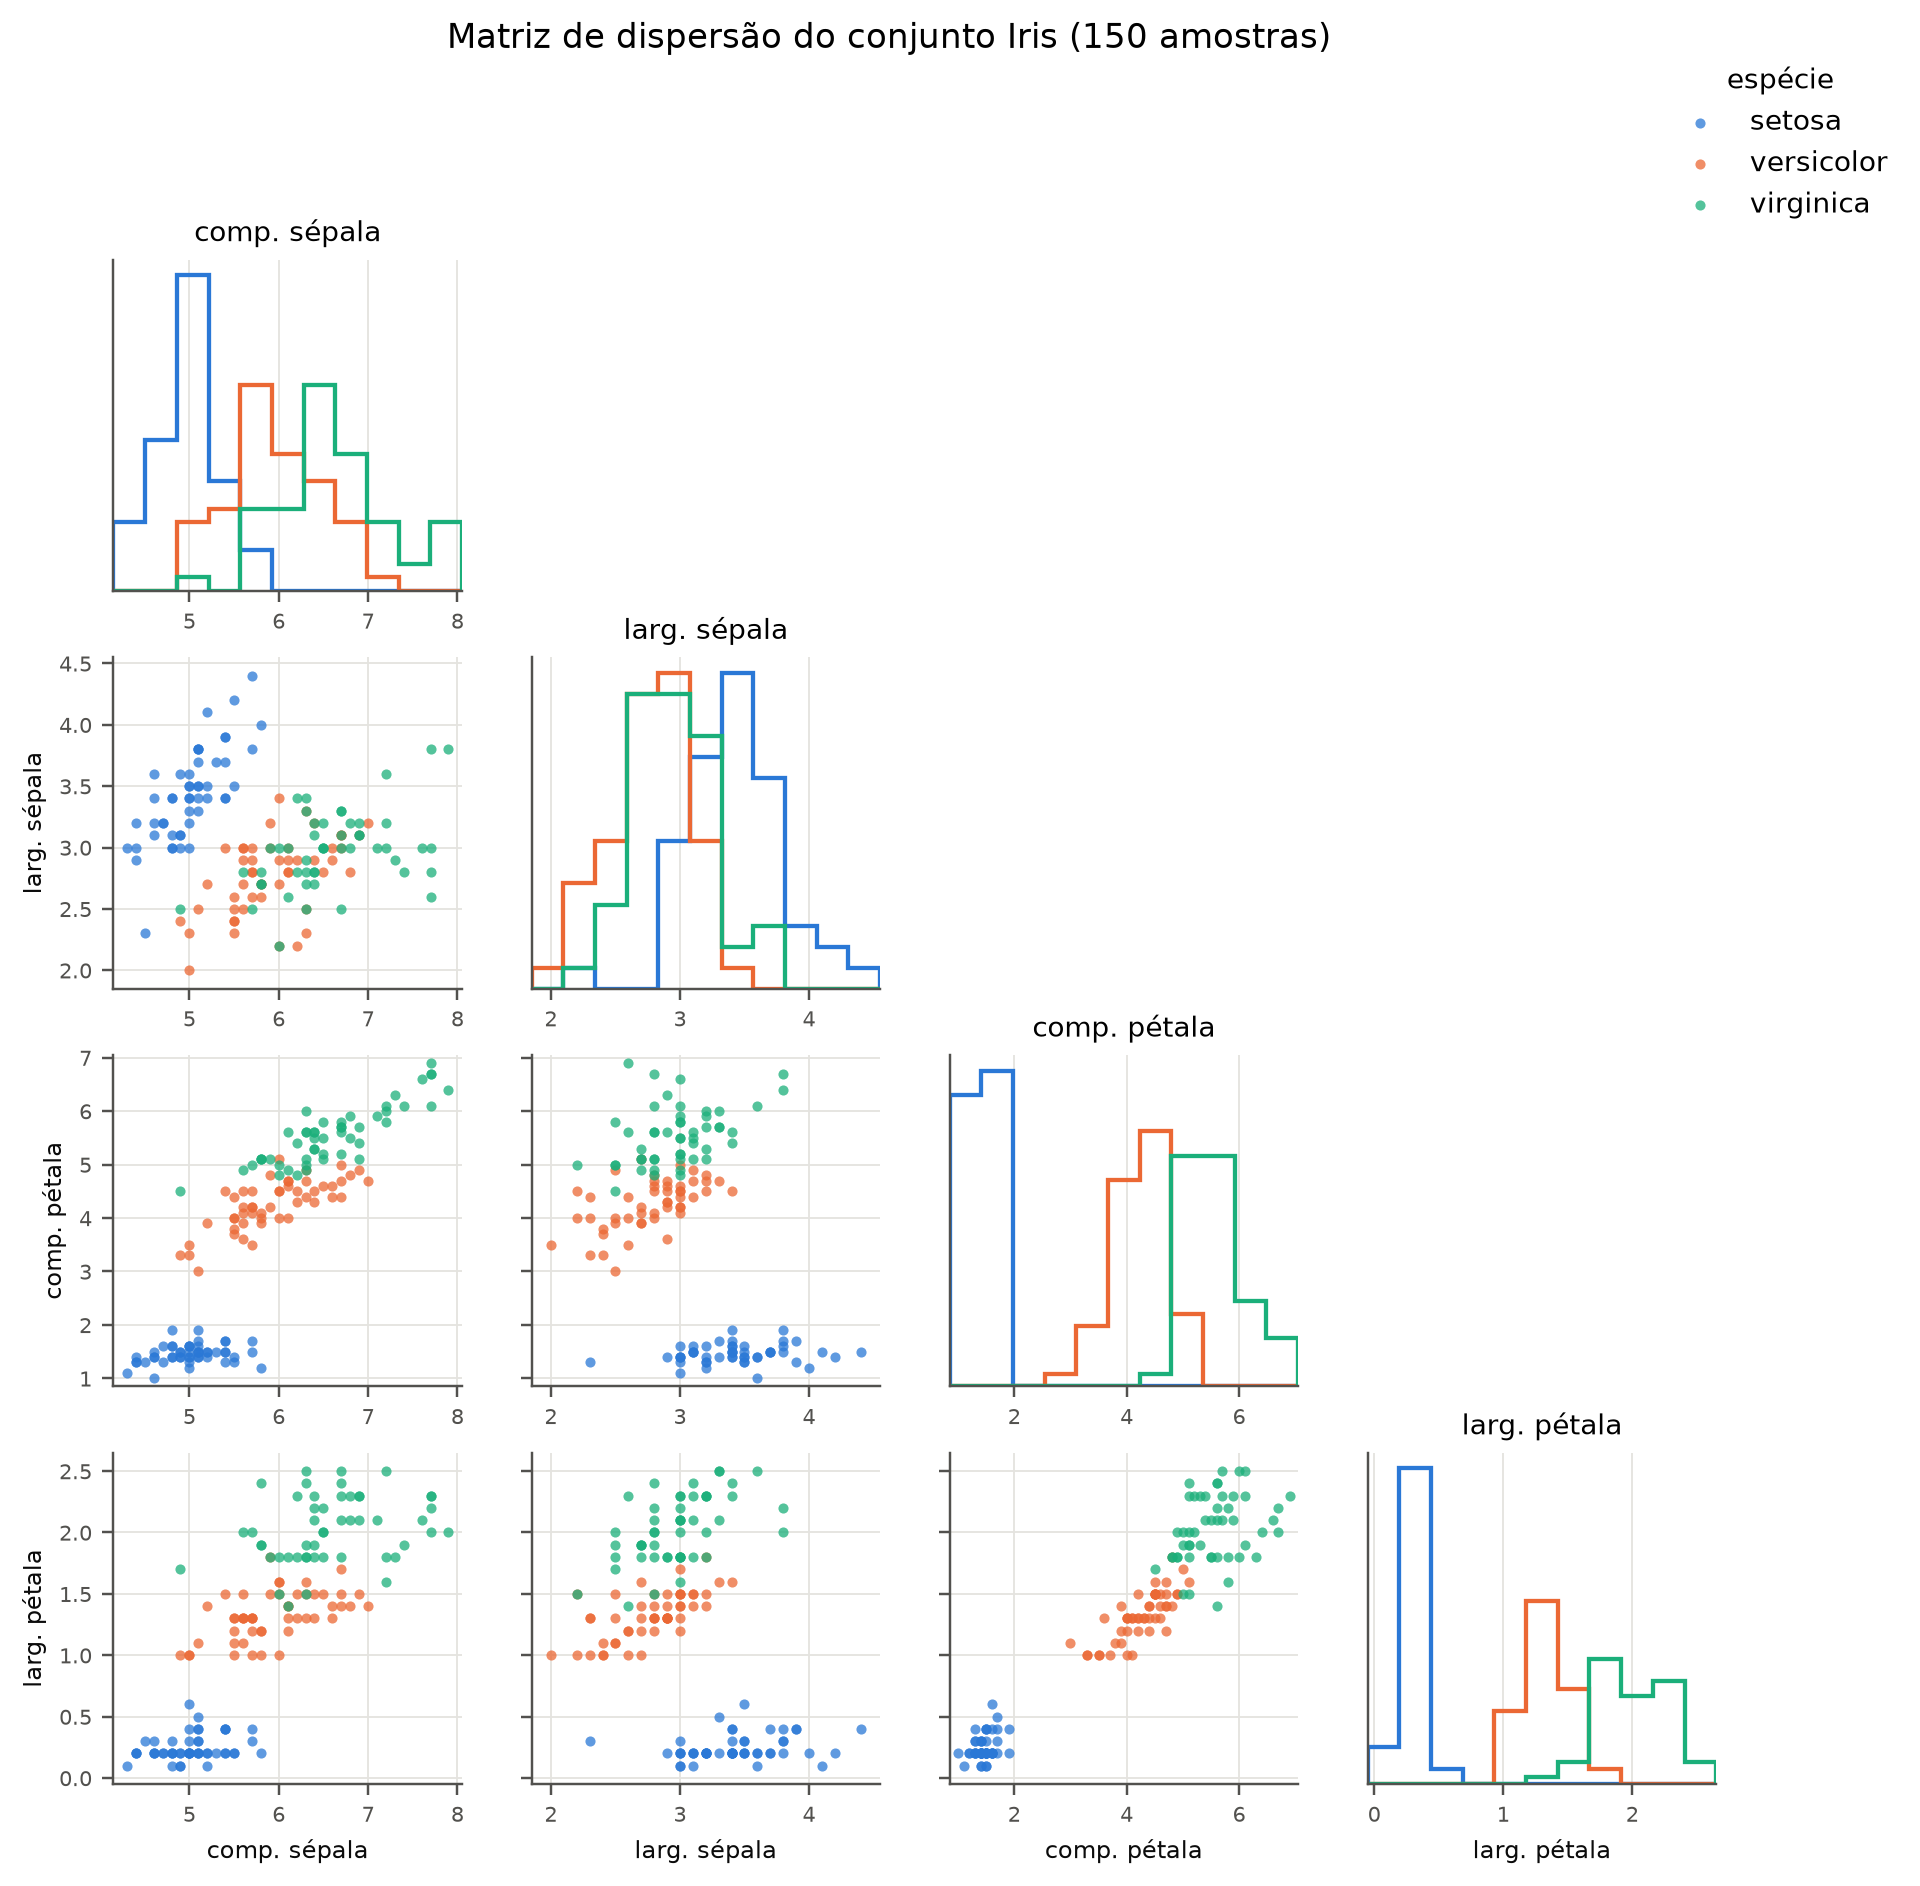
\includegraphics[width=0.72\textwidth]{fig_iris_dispersao.png}
	\caption{Matriz de dispersão dos quatro atributos. Abaixo da diagonal, dispersões dois a dois;
	na diagonal, histogramas por espécie. A \emph{setosa} (azul) forma um grupo isolado em todas as
	projeções que envolvem a pétala.}
	\label{fig:dispersao}
\end{figure}

\paragraph{A \emph{setosa} é separável.} Em qualquer gráfico que use comprimento ou largura da
pétala, os pontos azuis ocupam uma região própria, sem sobreposição com as demais espécies. Isso
significa que a classe é linearmente separável das outras duas: existe um hiperplano que a isola.

\paragraph{\emph{Versicolor} e \emph{virginica} se sobrepõem.} A fronteira entre as duas é difusa.
Há flores de \emph{versicolor} com pétalas tão grandes quanto as de \emph{virginica} e vice-versa.
Praticamente todo o erro de qualquer classificador razoável no Iris vem dessa região.

\paragraph{A sépala ajuda pouco.} A \figura{fig:boxplots} mostra que as distribuições de largura
da sépala das três espécies se sobrepõem quase completamente. O comprimento da sépala separa bem a
\emph{setosa}, mas confunde as outras duas. Em outras palavras: o problema tem duas variáveis
informativas e duas quase redundantes.

\begin{figure}[htbp]
	\centering
	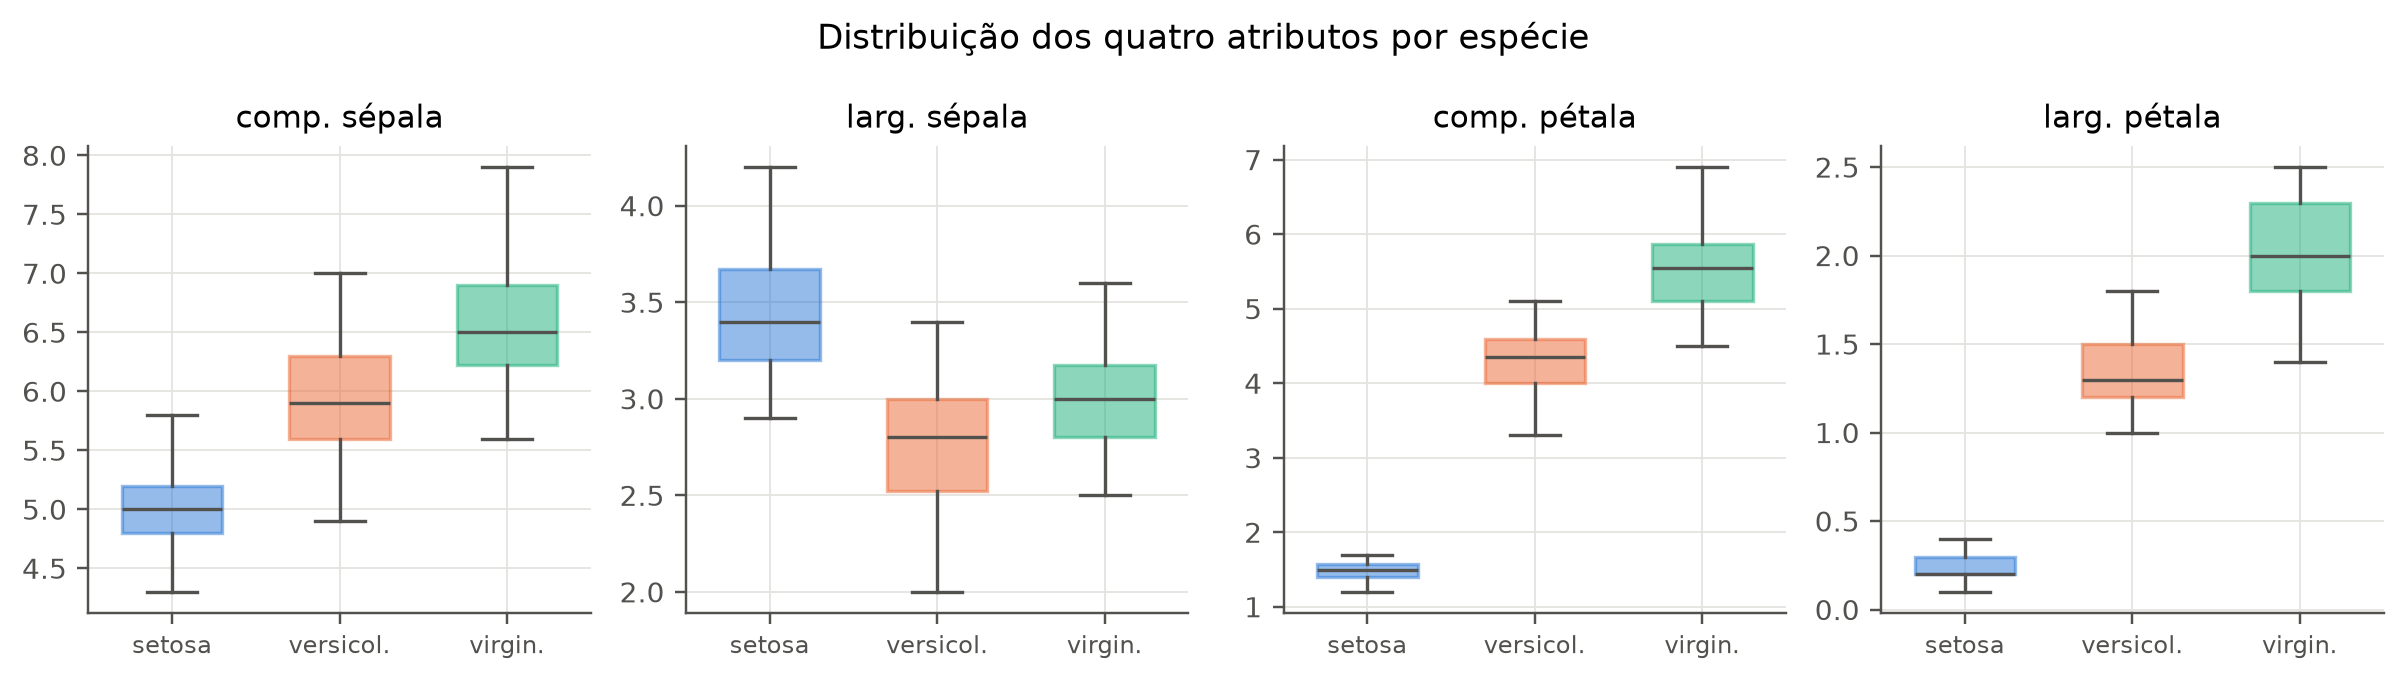
\includegraphics[width=\textwidth]{fig_iris_boxplots.png}
	\caption{Distribuições dos quatro atributos por espécie. As caixas vão do primeiro ao terceiro
	quartil, a linha central é a mediana e os bigodes se estendem até 1,5 vez o intervalo
	interquartil.}
	\label{fig:boxplots}
\end{figure}

A matriz de correlação (\figura{fig:correlacao}) confirma a leitura. Comprimento e largura da
pétala têm correlação de $0{,}96$; comprimento da sépala correlaciona $0{,}87$ com o comprimento da
pétala e $0{,}82$ com a largura da pétala. A largura da sépala é a variável mais independente:
$-0{,}43$ com o comprimento da pétala e $-0{,}37$ com a largura. Há, portanto, redundância
considerável: quatro medidas resumem essencialmente duas direções de variação.

\begin{figure}[htbp]
	\centering
	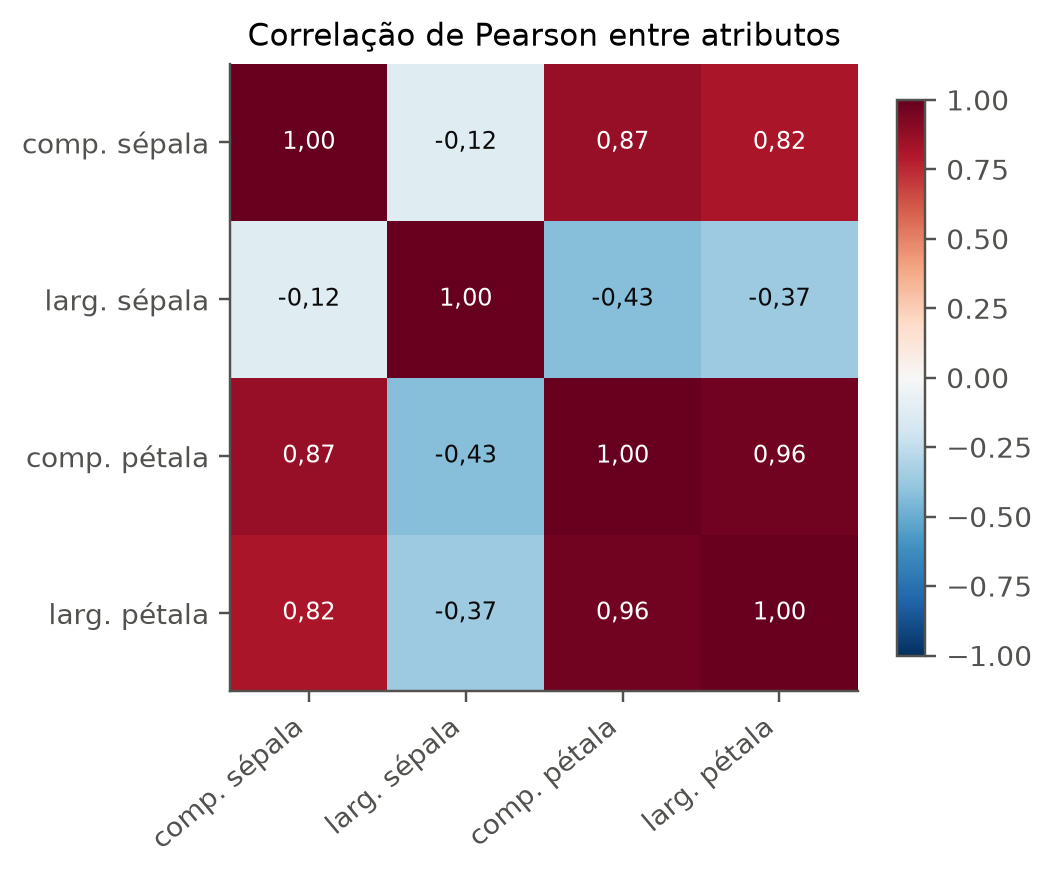
\includegraphics[width=0.62\textwidth]{fig_iris_correlacao.png}
	\caption{Correlação de Pearson entre os quatro atributos. Azul indica correlação positiva,
	vermelho, negativa.}
	\label{fig:correlacao}
\end{figure}

A análise de componentes principais torna essa redundância explícita. Depois de padronizar os
atributos, a primeira componente explica $73{,}0\,\%$ da variância e a segunda, $22{,}9\,\%$
(\figura{fig:pca}). Juntas, elas resumem $95{,}9\,\%$ da informação --- e, no plano formado por
elas, as três espécies aparecem em uma sequência ordenada, com a \emph{setosa} isolada à esquerda e
as outras duas ocupando uma faixa contínua à direita.

\begin{figure}[htbp]
	\centering
	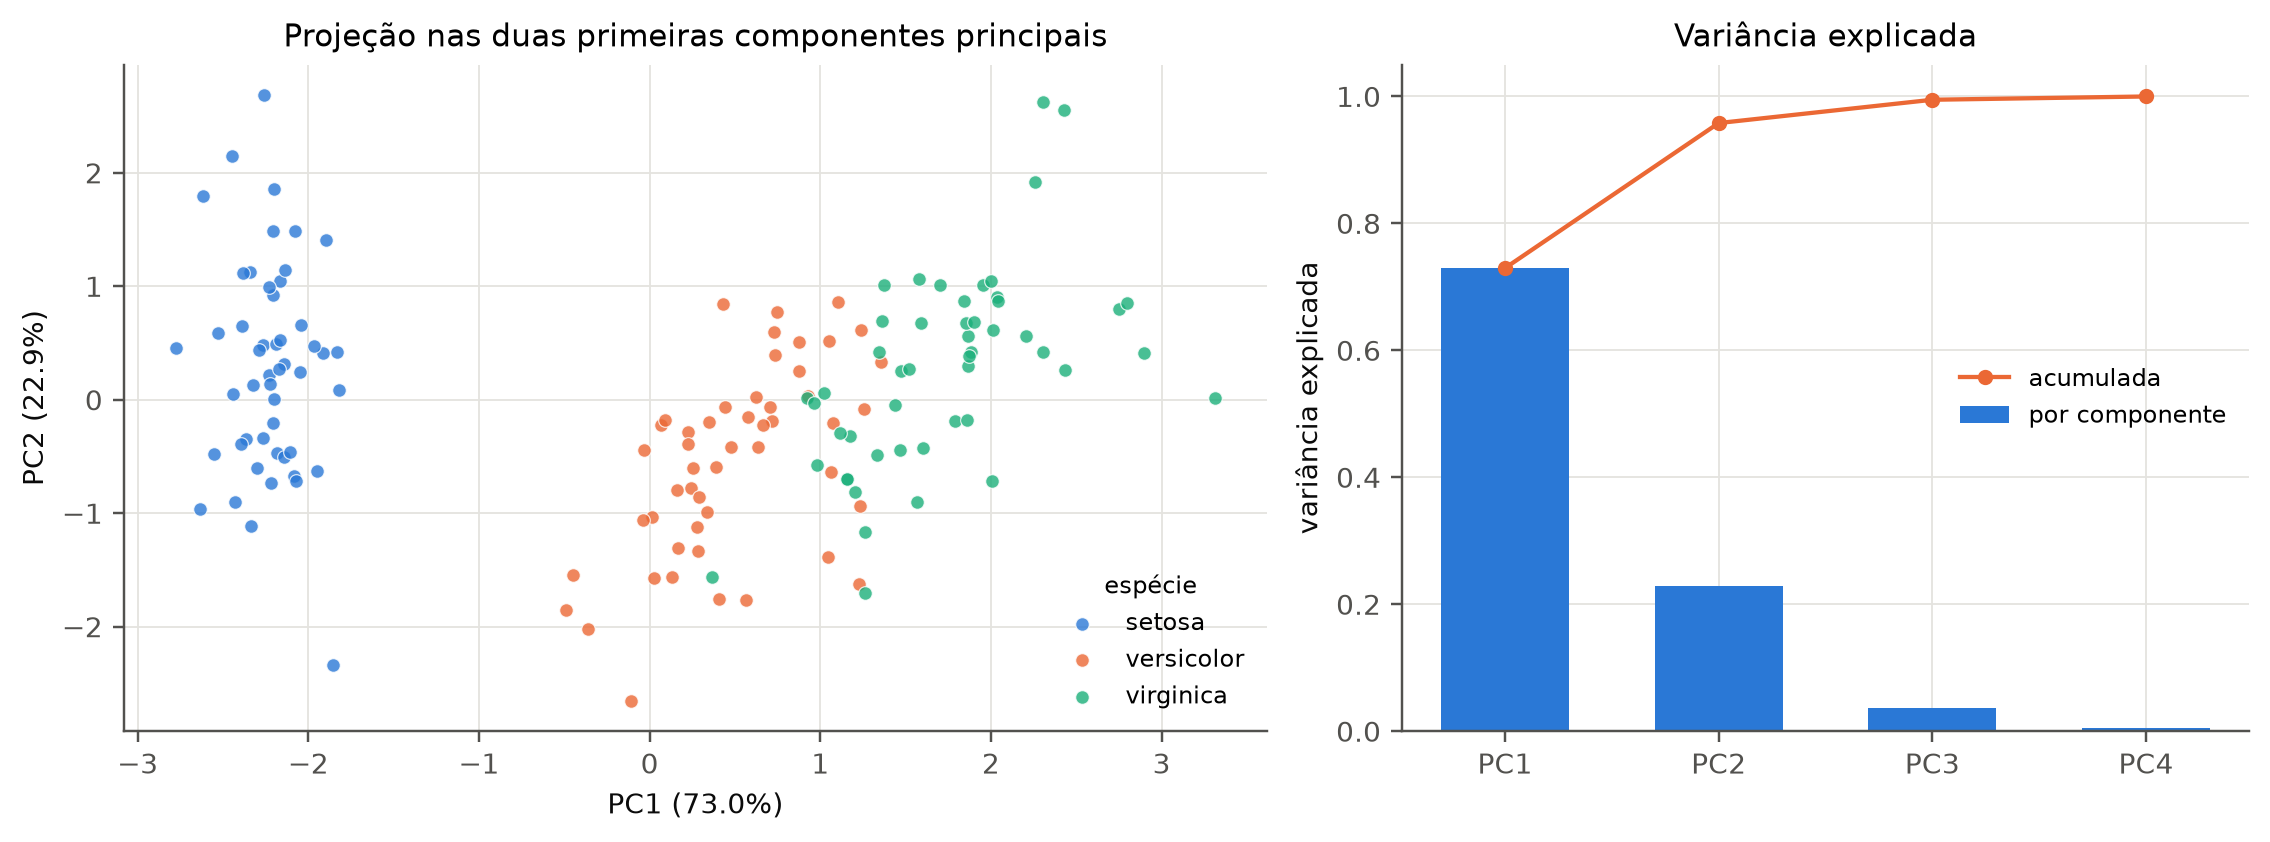
\includegraphics[width=\textwidth]{fig_iris_pca.png}
	\caption{Projeção nas duas primeiras componentes principais (atributos padronizados) e
	variância explicada por componente. A separação entre as espécies é quase inteiramente
	unidimensional.}
	\label{fig:pca}
\end{figure}

\subsection{O que esperar de um classificador}

A análise exploratória permite prever o desempenho antes de treinar qualquer modelo. Como a
\emph{setosa} é separável, espera-se acerto próximo de $100\,\%$ nessa classe. O erro deve se
concentrar na fronteira entre \emph{versicolor} e \emph{virginica}, onde alguns pontos são
ambiguos até para um especialista. Uma acurácia global entre $95\,\%$ e $98\,\%$ é o intervalo
plausível; muito acima disso sugere vazamento de informação ou sorte na divisão; muito abaixo
sugere erro de implementação.

Essa previsão é importante porque fornece um critério externo de sanidade. Quando um modelo
reporta $99{,}9\,\%$ em um conjunto com sobreposição visível, a primeira hipótese não é genialidade
do modelo, e sim algum problema no protocolo de avaliação --- por exemplo, padronizar os dados
antes de dividir treino e teste, ou ajustar hiperparâmetros no conjunto de teste.

\subsection{Limitações do conjunto}

O Iris é excelente para aprender, mas ruim para generalizar conclusões. Três limitações devem ser
registradas desde já.

\begin{itemize}
	\item \textbf{tamanho}: 150 amostras implicam intervalos de confiança largos. Um acerto a mais
	      ou a menos no conjunto de teste muda a acurácia em $2{,}2$ pontos percentuais;
	\item \textbf{dimensionalidade}: com quatro atributos e três classes, qualquer modelo tem
	      capacidade de sobra. O problema não testa a habilidade da rede de aprender representações
	      complexas;
	\item \textbf{quase separabilidade}: como as classes são quase linearmente separáveis, modelos
	      lineares competem de igual para igual com redes neurais, o que limita o que se pode
	      concluir sobre a vantagem de arquiteturas profundas.
\end{itemize}

Essas limitações não impedem o estudo da MLP; elas definem o que o estudo pode afirmar. O
\secao{sec:discussao} retoma o ponto com os resultados em mãos.
